\documentclass[11pt]{article}

%% MinionPro fonts 
%\usepackage[lf]{MinionPro}
%\usepackage{MnSymbol}
\usepackage{microtype}

%% Margins
\usepackage{geometry}
\geometry{verbose,letterpaper,tmargin=1in,bmargin=1in,lmargin=1in,rmargin=1in}

%% Other packages
\usepackage{amsmath}
\usepackage{amsthm}
\usepackage[shortlabels]{enumitem}
\usepackage{titlesec}
\usepackage{soul}
\usepackage{tikz}
\usepackage{mathtools}
\usepackage{pgfplots}
\usepackage{tikz-3dplot}
\usepackage{algorithmic}
\usepackage[export]{adjustbox}
\usepackage{tcolorbox}
\usepackage{optprog}

%% Paragraph style settings
\setlength{\parskip}{\medskipamount}
\setlength{\parindent}{0pt}

%% Change itemize bullets
\renewcommand{\labelitemi}{$\bullet$}
\renewcommand{\labelitemii}{$\circ$}
\renewcommand{\labelitemiii}{$\diamond$}
\renewcommand{\labelitemiv}{$\cdot$}

%% Colors
\definecolor{rred}{RGB}{204,0,0}
\definecolor{ggreen}{RGB}{0,145,0}
\definecolor{yyellow}{RGB}{255,185,0}
\definecolor{bblue}{rgb}{0.2,0.2,0.7}
\definecolor{ggray}{RGB}{190,190,190}
\definecolor{ppurple}{RGB}{160,32,240}
\definecolor{oorange}{RGB}{255,165,0}

%% Shrink section fonts
\titleformat*{\section}{\normalsize\bf}
\titleformat*{\subsection}{\normalsize\bf}
\titleformat*{\subsubsection}{\normalsize\it}

% %% Compress the spacing around section titles
\titlespacing*{\section}{0pt}{1.5ex}{0.75ex}
\titlespacing*{\subsection}{0pt}{1ex}{0.5ex}
\titlespacing*{\subsubsection}{0pt}{1ex}{0.5ex}

%% amsthm settings
\theoremstyle{definition}
\newtheorem{problem}{Problem}
\newtheorem{example}{Example}
\newtheorem*{theorem}{Theorem}
\newtheorem*{bigthm}{Big Theorem}
\newtheorem*{biggerthm}{Bigger Theorem}
\newtheorem*{bigcor1}{Big Corollary 1}
\newtheorem*{bigcor2}{Big Corollary 2}

%% tikz settings
\usetikzlibrary{calc}
\usetikzlibrary{patterns}
\usetikzlibrary{decorations}
\usepgfplotslibrary{polar}

%% algorithmic setup
\algsetup{linenodelimiter=}
\renewcommand{\algorithmiccomment}[1]{\quad// #1}
\renewcommand{\algorithmicrequire}{\emph{Input:}}
\renewcommand{\algorithmicensure}{\emph{Output:}}

%% Answer box macros
%% \answerbox{alignment}{width}{height}
\newcommand{\answerbox}[3]{%
  \fbox{%
    \begin{minipage}[#1]{#2}
      \hfill\vspace{#3}
    \end{minipage}
  }
}

%% \answerboxfull{alignment}{height}
\newcommand{\answerboxfull}[2]{%
  \answerbox{#1}{6.38in}{#2} 
}

%% \answerboxone{alignment}{height} -- for first-level bullet
\newcommand{\answerboxone}[2]{%
  \answerbox{#1}{6.0in}{#2} 
}

%% \answerboxtwo{alignment}{height} -- for second-level bullet
\newcommand{\answerboxtwo}[2]{%
  \answerbox{#1}{5.8in}{#2}
}

%% special boxes
\newcommand{\wordbox}{\answerbox{c}{1.2in}{.7cm}}
\newcommand{\catbox}{\answerbox{c}{.5in}{.7cm}}
\newcommand{\letterbox}{\answerbox{c}{.7cm}{.7cm}}

%% Miscellaneous macros
\newcommand{\tstack}[1]{\begin{multlined}[t] #1 \end{multlined}}
\newcommand{\cstack}[1]{\begin{multlined}[c] #1 \end{multlined}}
\newcommand{\ccite}[1]{\only<presentation>{{\scriptsize\color{gray} #1}}\only<article>{{\small [#1]}}}
\newcommand{\grad}{\nabla}
\newcommand{\ra}{\ensuremath{\rightarrow}~}
\newcommand{\maximize}{\text{maximize}}
\newcommand{\minimize}{\text{minimize}}
\newcommand{\subjectto}{\text{subject to}}
\newcommand{\trans}{\mathsf{T}}
\newcommand{\bb}{\mathbf{b}}
\newcommand{\bx}{\mathbf{x}}
\newcommand{\bc}{\mathbf{c}}
\newcommand{\bd}{\mathbf{d}}
\newcommand{\blu}{\color{blue}}

%% LP format
%    \begin{align*}
%      \maximize \quad & \mathbf{c}^{\trans} \mathbf{x}\\
%      \subjectto \quad & A \mathbf{x} = \mathbf{b}\\
%                       & \mathbf{x} \ge \mathbf{0}
%    \end{align*}


%% Redefine maketitle
\makeatletter
\renewcommand{\maketitle}{
  \noindent SA405 -- AMP \hfill Rader \#2.42 \\

  \begin{center}\Large{\textbf{\@title}}\end{center}
}
\makeatother

%% ----- Begin document ----- %%
\begin{document}
  
\title{HW3: Network Flows part 2}


\maketitle

\textbf{Problem 1:} Seven types of packages are to be delivered by five trucks. There are three packages of each type, and the capacities of the five trucks are 6, 4, 5, 4, and 3 packages, respectively. Set up a maximum-flow problem that can be used to determine whether the packages can be loaded so that no truck carries two packages of the same type. 

\begin{enumerate}
\item Draw the network diagram for this problem. \emph{Hint: Draw a source and sink node. The source node should be connected to each of the 7 packages and the sink node should be connected to each of the trucks.}

\begin{center}
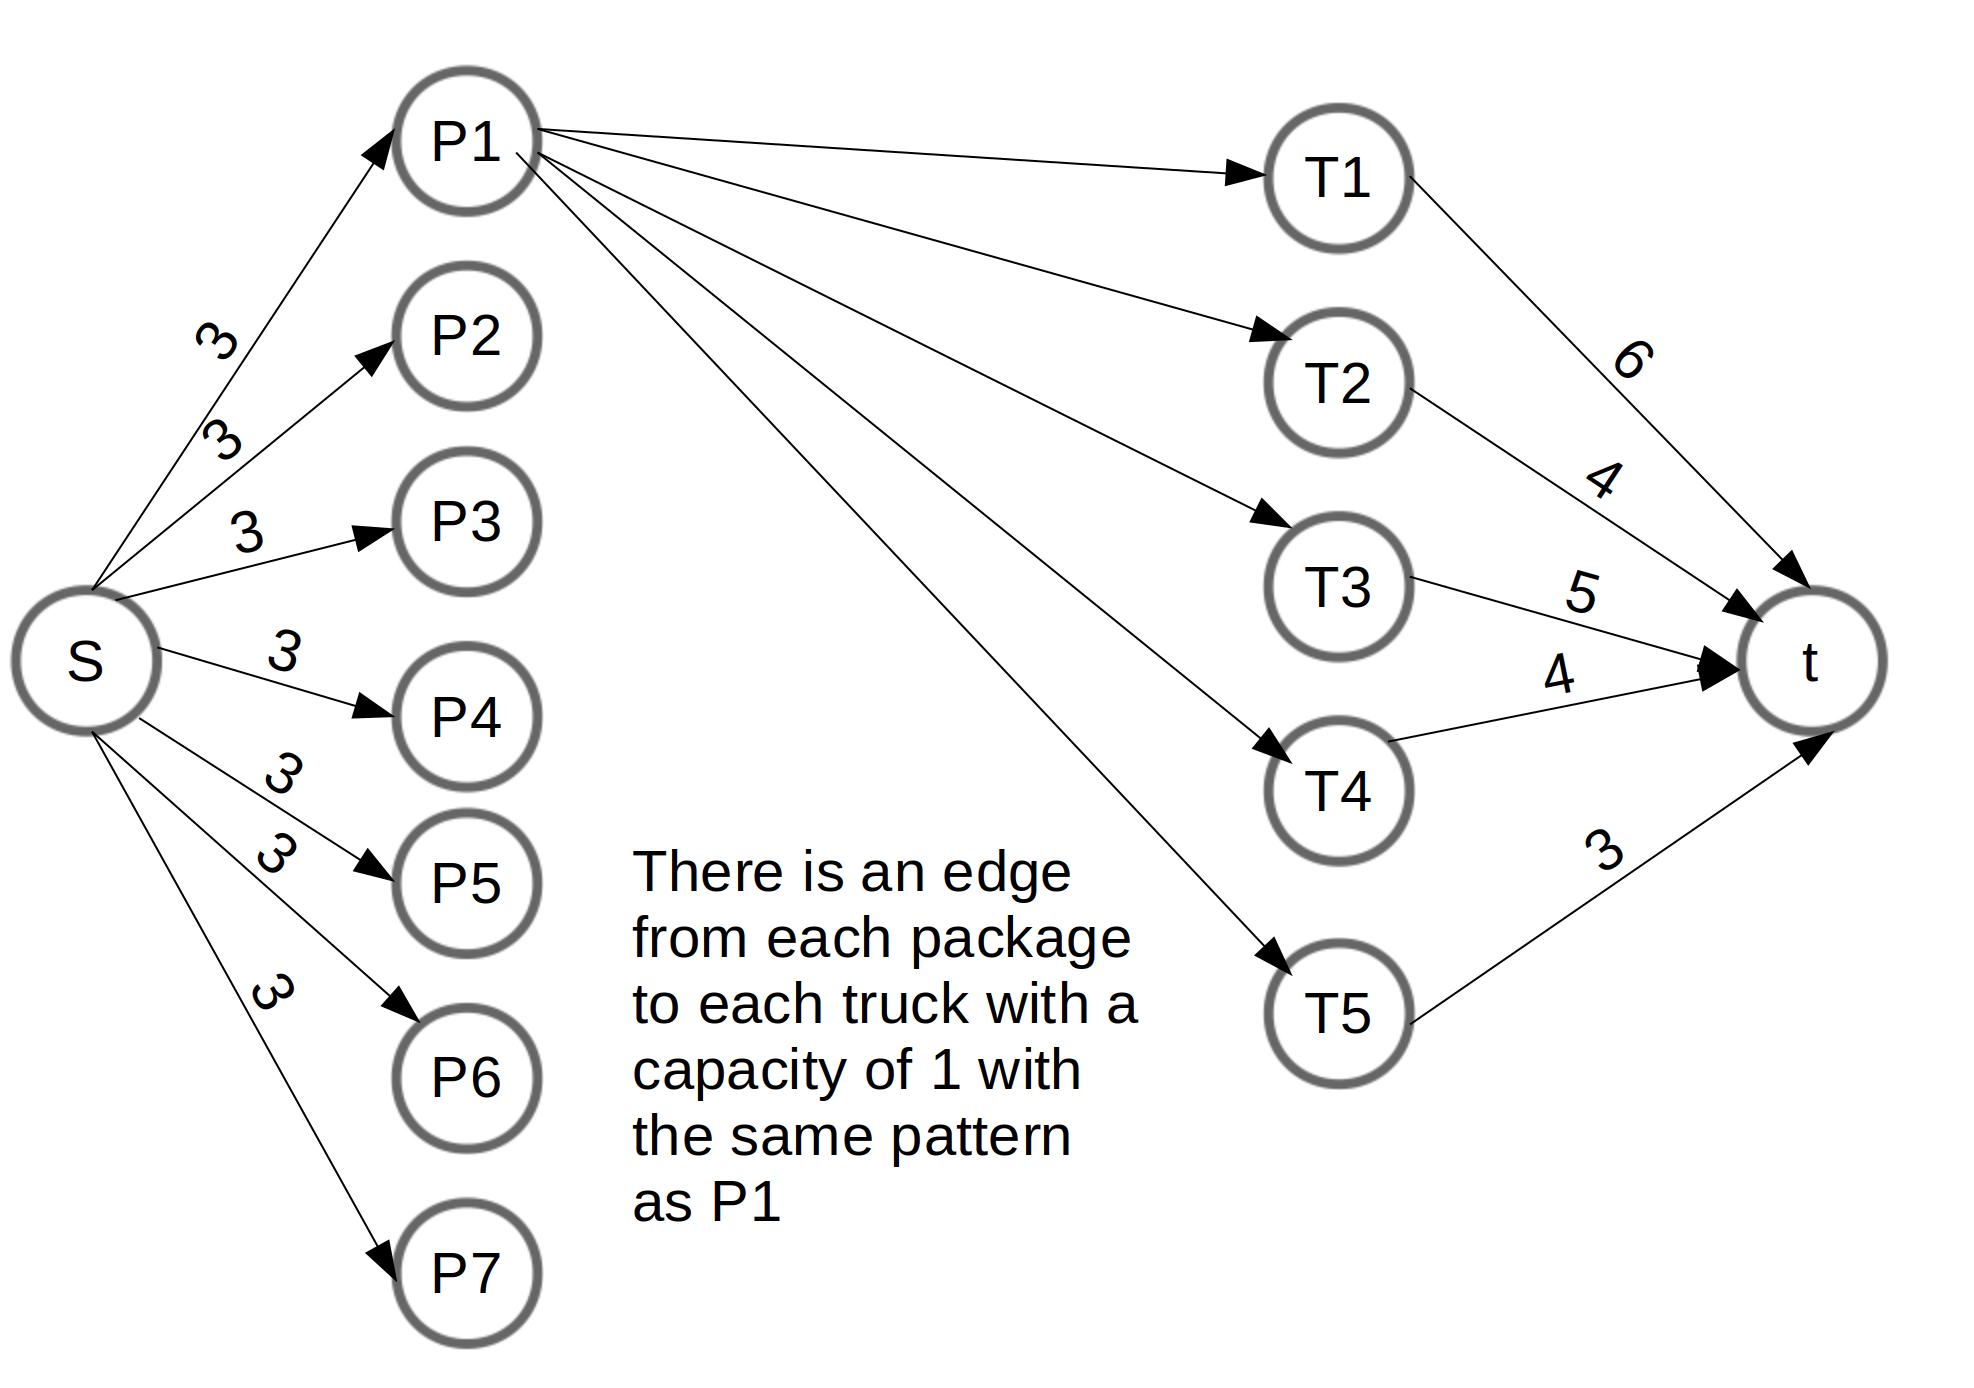
\includegraphics[width=0.9\textwidth]{Prob1.png}
\end{center}

\newpage

\item Formulate a concrete max flow model that can determine whether the packages can be loaded so that no truck carries two packages of the same type.

{\blu
\textbf{\underline{Decision Variables}}

Let $x_{s,p1}$ be the flow from S to P1

Let $x_{s,p2}$ be the flow from S to P2

$\vdots$

Let $x_{t5,t}$ be the flow from T5 to t

\textbf{\underline{Objective Function}}

\[
\text{max flow } x_{s,p1}+x_{s,p2} + \cdots + x_{s,p7}
\]


\textbf{\underline{Constraints}}

There's about 50 capacity constraints and 14 flow balance constraints. I'm going to write a few of them for the solution

\begin{optprog*}
st & x_{s,p1} & \leq & 3 & \text{(Capacity of edge $(s,p1)$)} \\
   & x_{s,p2} & \leq & 3 & \text{(Capacity of edge $(s,p2)$)} \\
   & \vdots \\
   & x_{t5,t} & \leq & 3 & \text{(Capacity of edge $(t5,t)$)} \\
   & x_{s,p1} & = & x_{p1,t1}+x_{p1,t2}+x_{p1,t3}+x_{p1,t4}+x_{p1,t5} & \text{(flow balance node P1)} \\
   & x_{s,p2} & = & x_{p2,t1}+x_{p2,t2}+x_{p2,t3}+x_{p2,t4}+x_{p2,t5} & \text{(flow balance node P2)} \\
   & \vdots \\
   & x_{p1,t5} + x_{p2,t5} + \cdots + x_{p7,t5} & = & x_{t5,t} & \text{(flow balance node T5)} \\
   & x_{s,p1} , x_{s,p2}, \cdots, x_{t5,t} & \geq & 0
\end{optprog*}


}

\end{enumerate}

\newpage

\textbf{Problem 2:}
(Adapted from Exercise 2.42, p 83) Consider the directed graph, $G = (V, E)$, given below, where each edge $(i,j) \in E$ has associated with it a distance $d_{i,j}$. Assume that node 1 is the source of the network. Our goal is to find the shortest path from node 1 to every other node in the network.


\begin{center} 
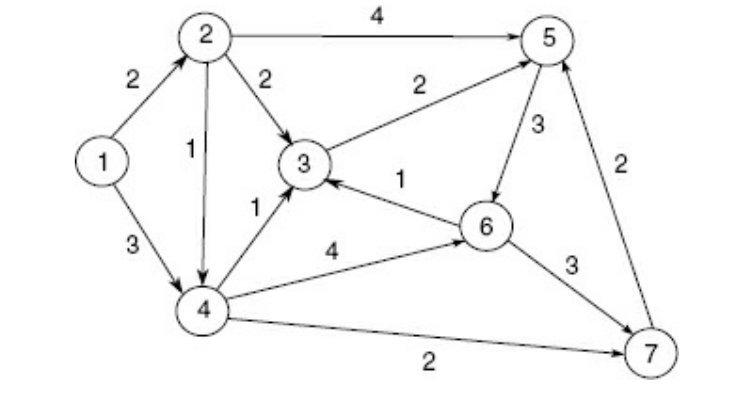
\includegraphics[width=0.9\textwidth]{ShortestPath.png}
\end{center}


\begin{enumerate}
\item Formulate the concrete model whose solution gives the shortest path from node 1 to every other node in the network.

{\blu
This problem is challenging, the easiest way to think about it is in terms of supply and demand. Basically, the supply of node 1 is ``6 shortest paths'' while the demand of nodes 2-7 is 1 shortest path. I believe there are more than 1 formulation of this problem but below is the most straightforward one.

\textbf{\underline{Decision Variables}}

Let $x_{1,2}$ be the number of times edge (1,2) is used in a shortest path

Let $x_{1,4}$ be the number of times edge (1,4) is used in a shortest path

$\vdots$

Let $x_{6,7}$ be the number of times edge (6,7) is used in a shortest path

\textbf{\underline{Objective Function}}

\[
\text{min cost } 2 x_{1,2} + 3 x_{1,4} + \cdots + 3 x_{6,7}
\]


\textbf{\underline{Constraints}}

The only necessary constraints are flow balance. Remember always that we have supply $+$ flow in $=$ demand $+$ flow out

\begin{optprog*}
st & 6 & = & x_{1,2} + x_{1,4} & \text{(flow balance at node 1)} \\
   & x_{1,2} & = & x_{2,3}+x_{2,4} + 1 & \text{(flow balance at node 2)} \\
   & x_{2,3} + x_{4,3} + x_{6,3} & = & x_{3,5}+ 1 & \text{(flow balance at node 3)} \\
   & x_{1,4} + x_{2,4} & = & x_{4,3}+x_{4,6} + 1 & \text{(flow balance at node 4)} \\
   & x_{2,5} + x_{3,5} + x_{7,5} & = & x_{5,6}+ 1 & \text{(flow balance at node 5)} \\
   & x_{4,6} + x_{5,6} & = & x_{6,3}+x_{6,7} + 1 & \text{(flow balance at node 6)} \\
   & x_{4,7} + x_{6,7} & = & x_{7,5}+ 1 & \text{(flow balance at node 7)} \\
   & x_{1,2}, x_{1,4}, \hdots, x_{7,5} & \geq & 0 
\end{optprog*}


}


\item Convert the concrete model from part (1) into a parameterized model.
\end{enumerate}

{\blu

\textbf{\underline{Sets}}

Let $N$ be the set of nodes

Let $E$ be the set of edges

\textbf{\underline{Decision Variables}}

Let $x_{i,j}$ be the number of times edge $(i,j)$ is used in a shortest path for all $(i,j) \in E$

\textbf{\underline{Parameters}}

Let $c_{i,j}$ be the cost of edge $(i,j)$ for all $(i,j) \in E$ 

Let $s_n$ be the supply of node $n$ for each $n \in N$ \emph{Note that this is 6 for node 1 and 0 for all other nodes}

Let $d_n$ be the demand of node $n$ for each $n \in N$ \emph{Note that this is 0 for node 1 and 1 for all other nodes}

\textbf{\underline{Objective Function}}

\[
\text{min cost } \sum_{(i,j) \in E} c_{i,j} x_{i,j}
\]


\textbf{\underline{Constraints}}

\begin{optprog*}
st & s_n + \sum_{(i,n) \in E} x_{i,n} & = & d_n + \sum_{(n,j) \in E} x_{n,j} & \text{for all $n \in N$} &  \text{(flow balance)} \\
  & x_{i,j} & \geq & 0 & \text{For all $(i,j) \in E$}
\end{optprog*}


}



\end{document}
